\documentclass[12pt]{article}
\usepackage[pdftex]{graphicx}
\usepackage{fullpage}

\begin{document}
\begin{center}
\textbf{filename: \expandafter\detokenize\expandafter{\myvar}}
\textbf{Window Size: \expandafter\detokenize\expandafter{\window}}

\textbf{Plots where the magnitudes are the direct output of the FFT}
\end{center}

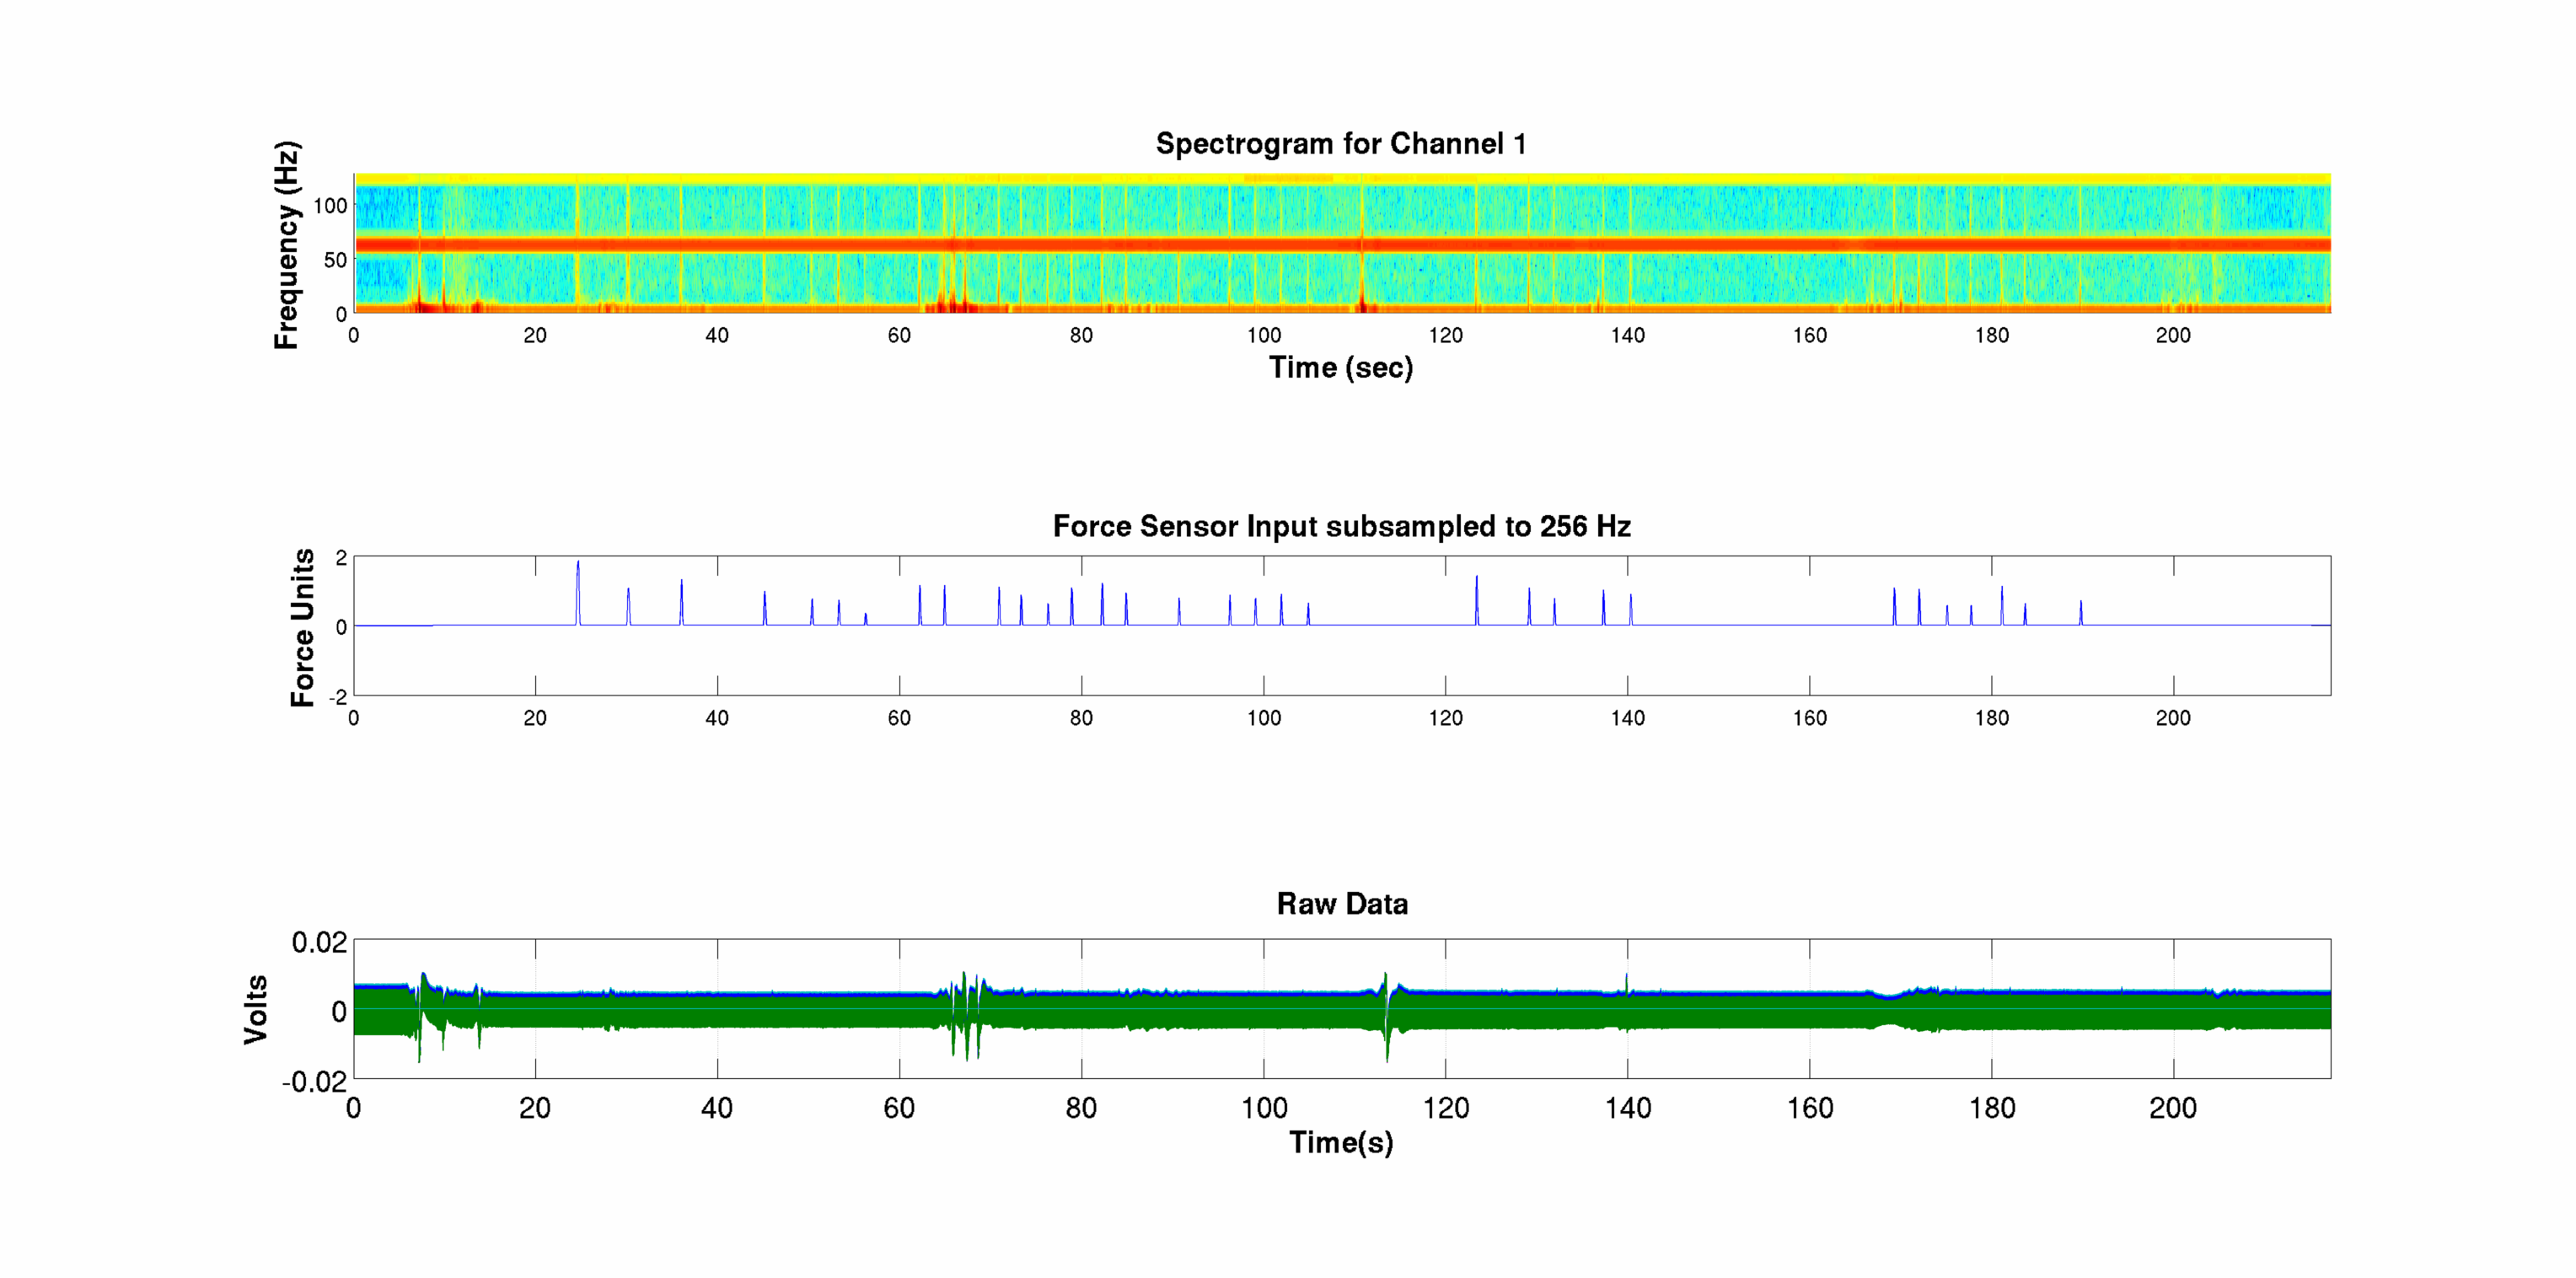
\includegraphics[scale=0.14]{raw_data_spectrogram.png}

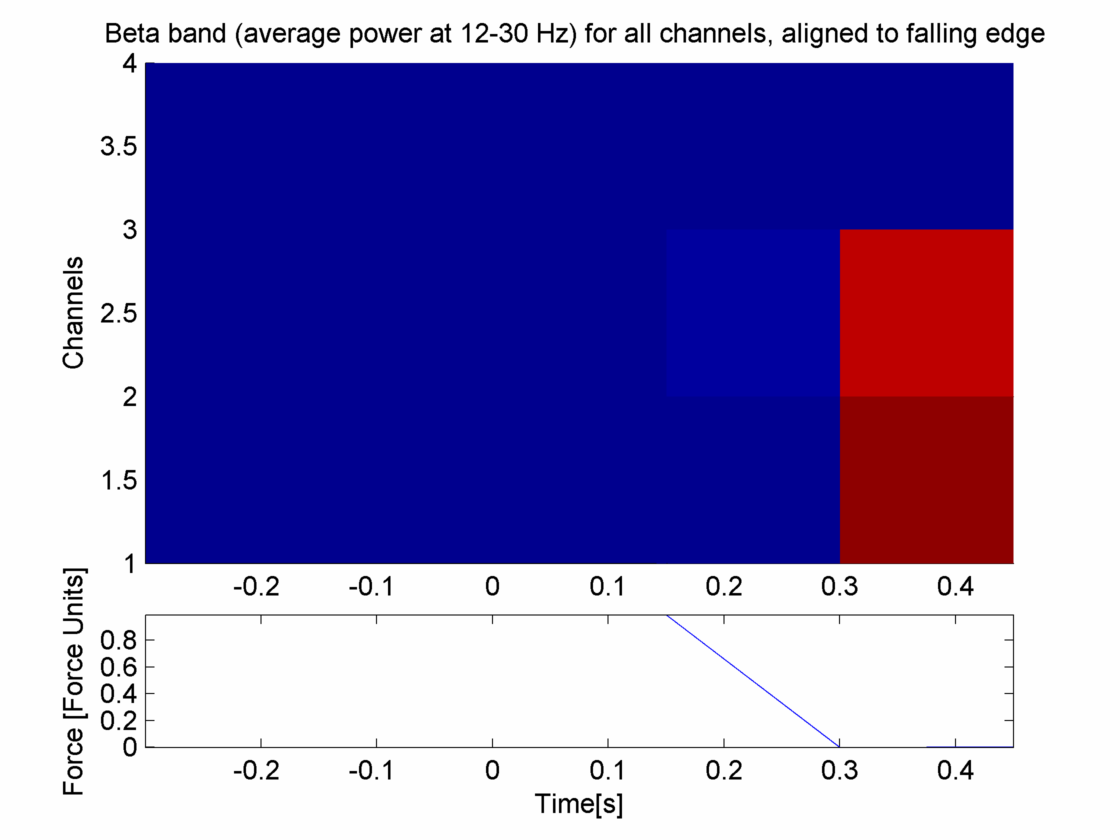
\includegraphics[scale=0.2]{beta_falling.png}
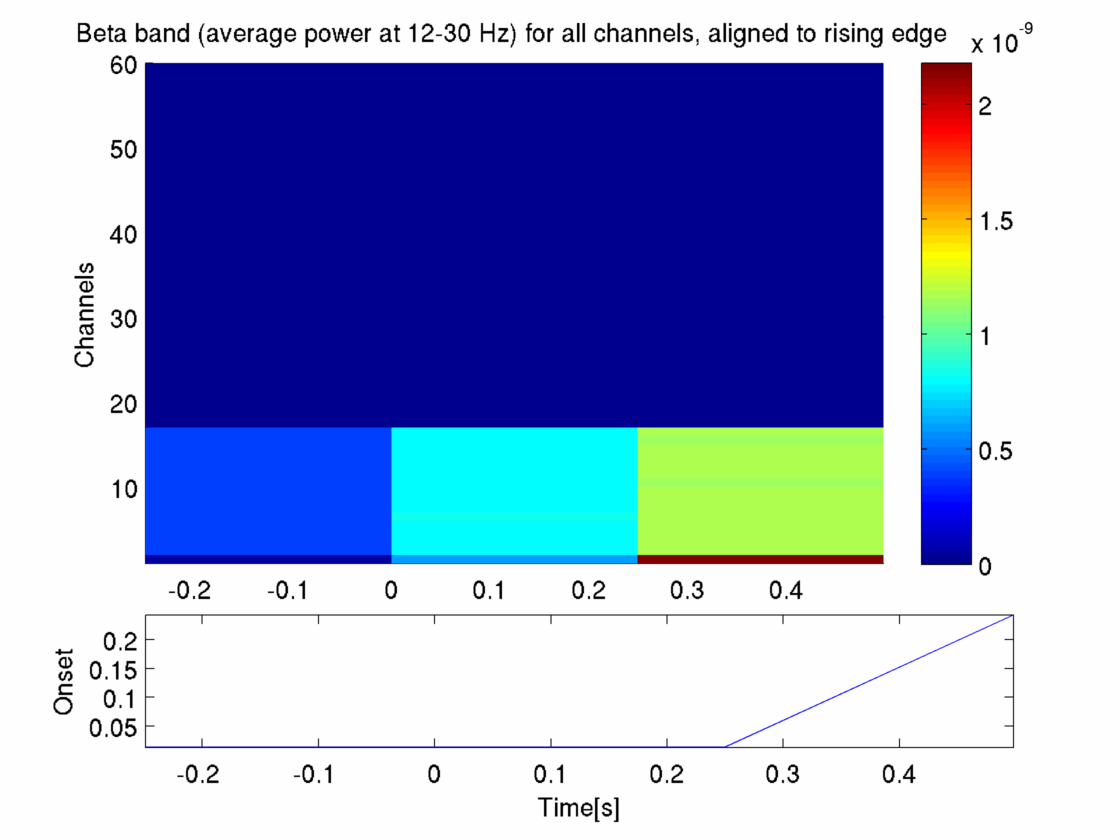
\includegraphics[scale=0.2]{beta_rising.png}

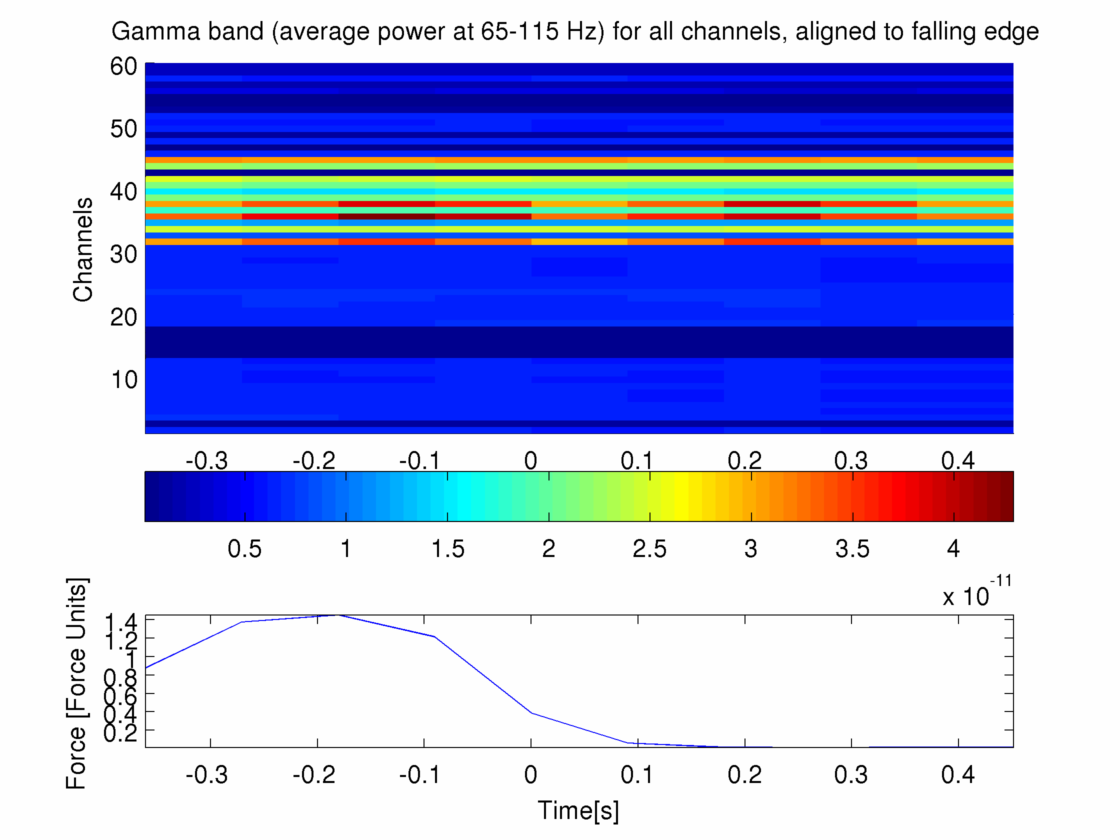
\includegraphics[scale=0.2]{gamma_falling.png}
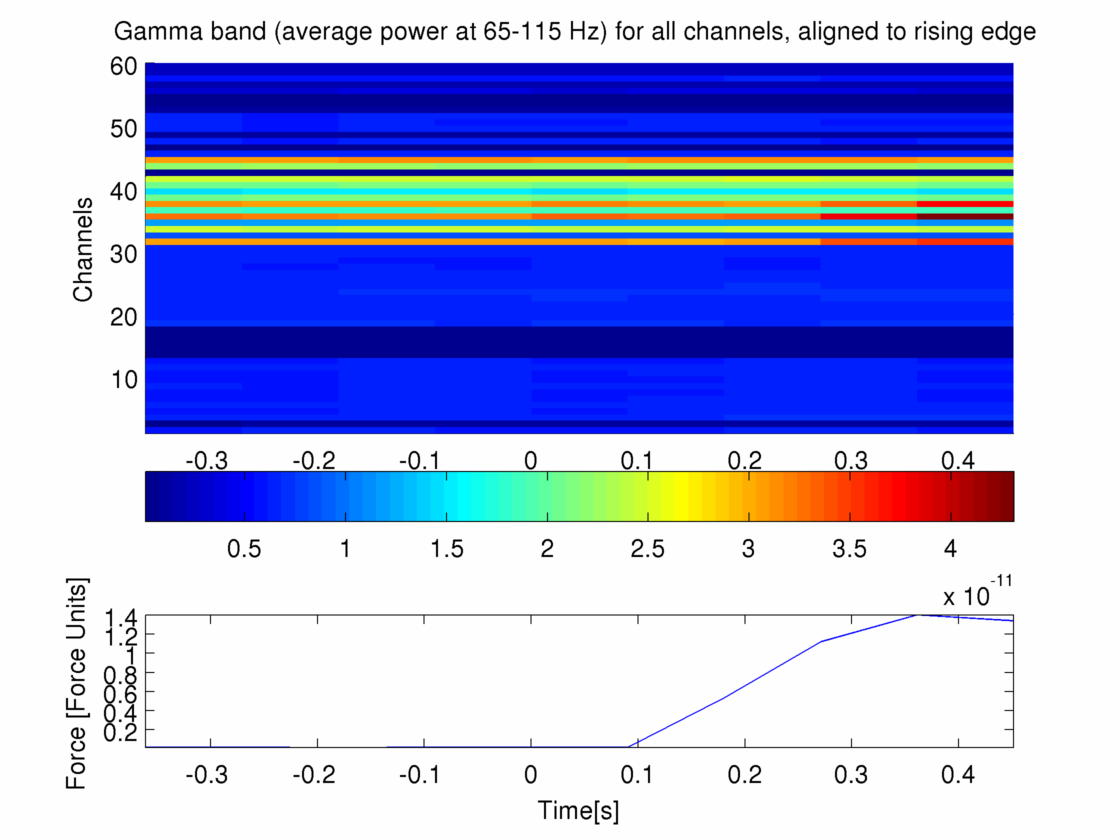
\includegraphics[scale=0.2]{gamma_rising.png}

\newpage

\begin{center}
\textbf{filename: \expandafter\detokenize\expandafter{\myvar}}

\textbf{Window Size: \expandafter\detokenize\expandafter{\window}}

\textbf{Plots where the magnitudes are the direct output of the FFT}
\end{center}

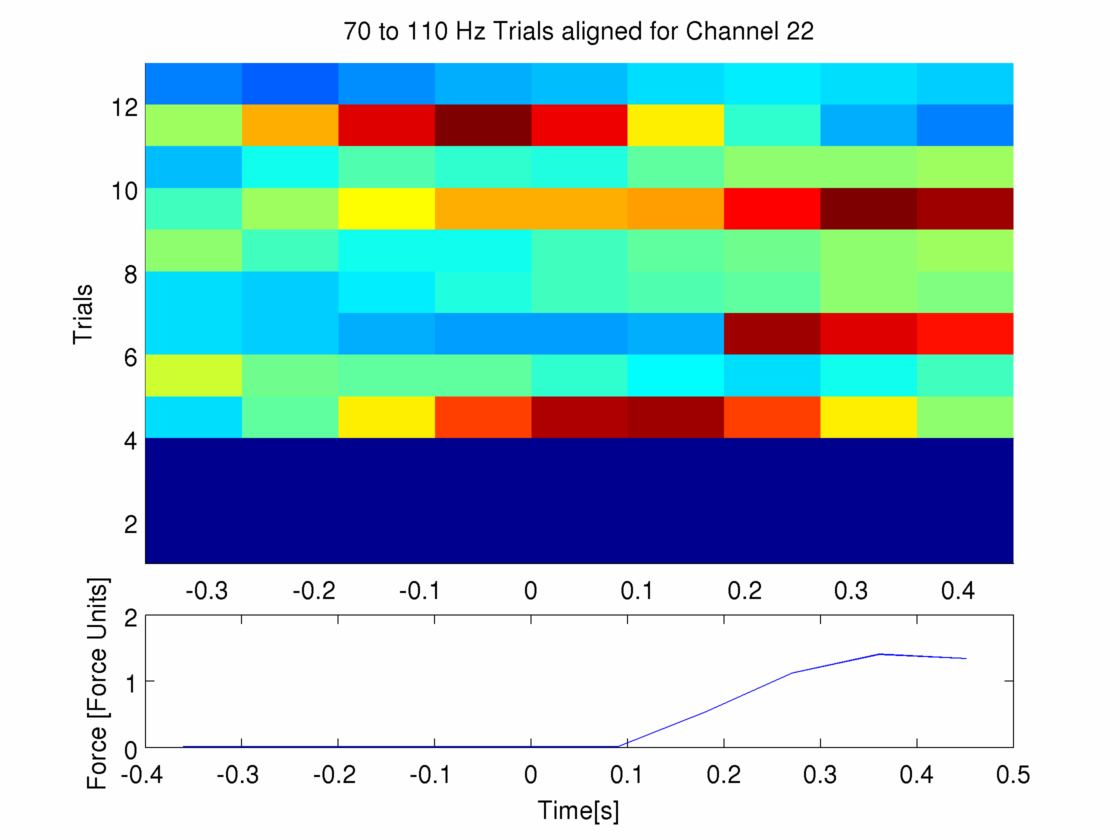
\includegraphics[scale=0.2]{plot_1_aligned_trials.png}
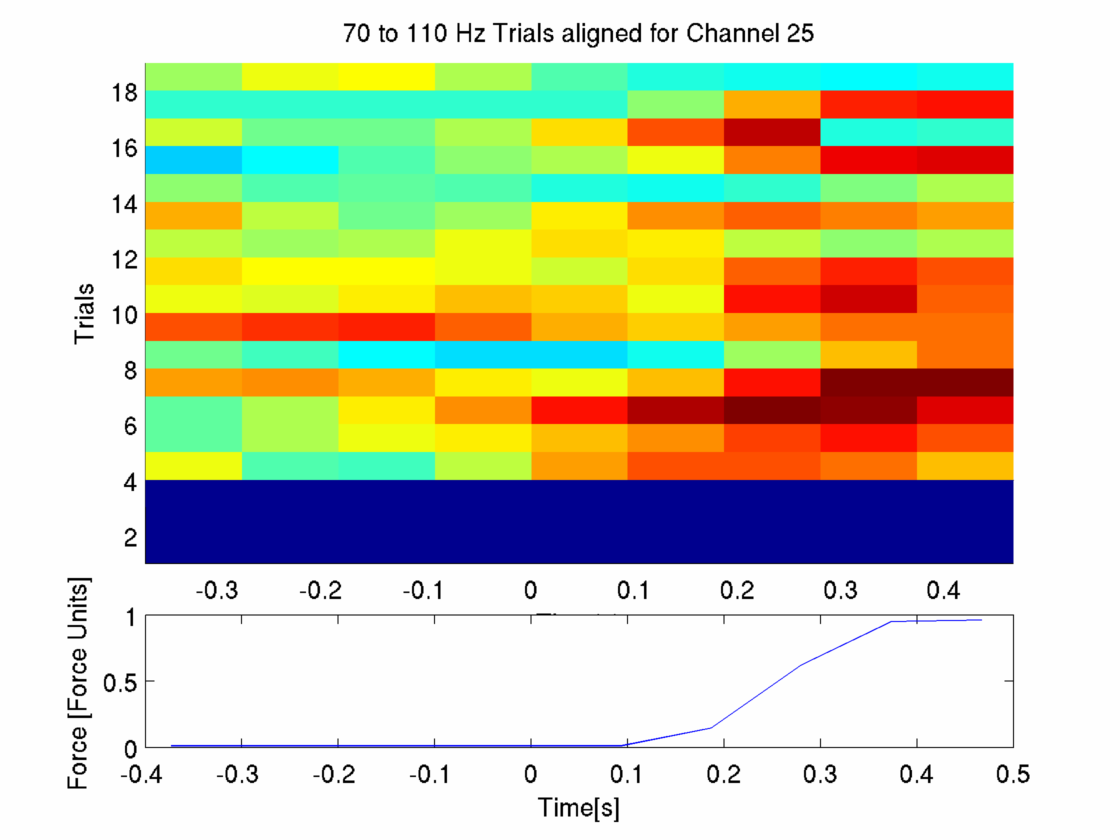
\includegraphics[scale=0.2]{plot_2_aligned_trials.png}

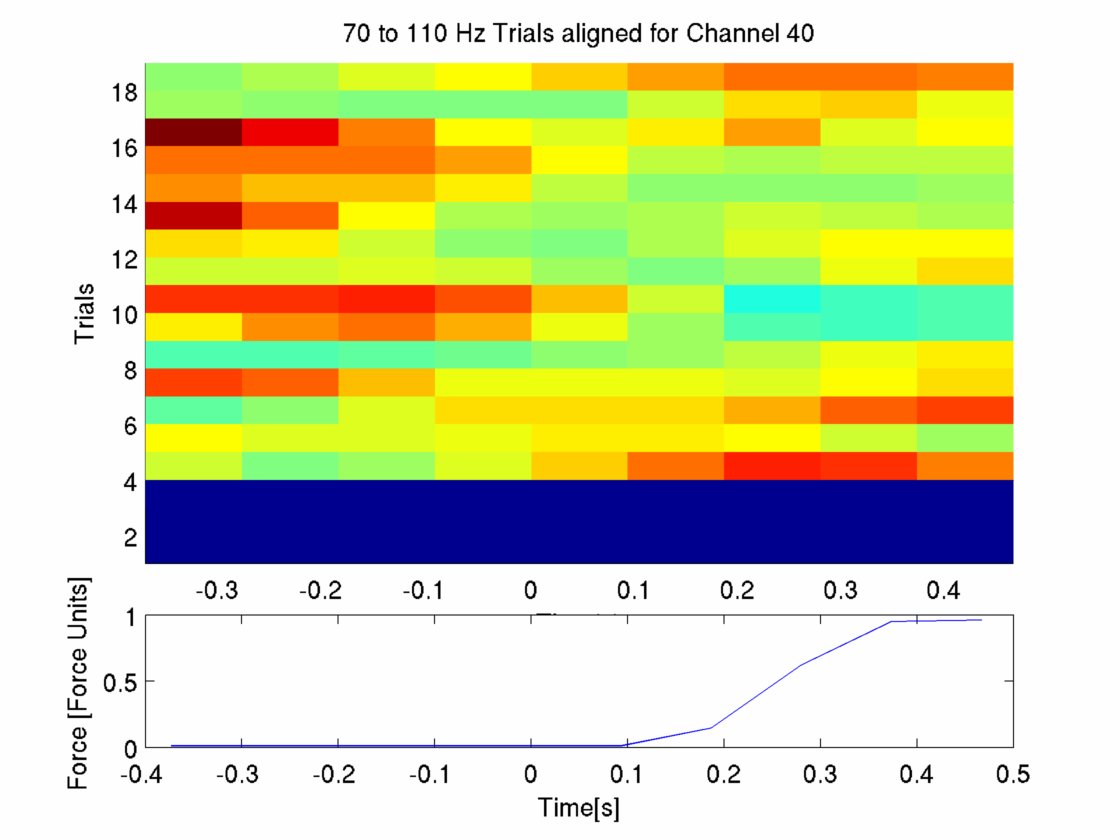
\includegraphics[scale=0.2]{plot_3_aligned_trials.png}
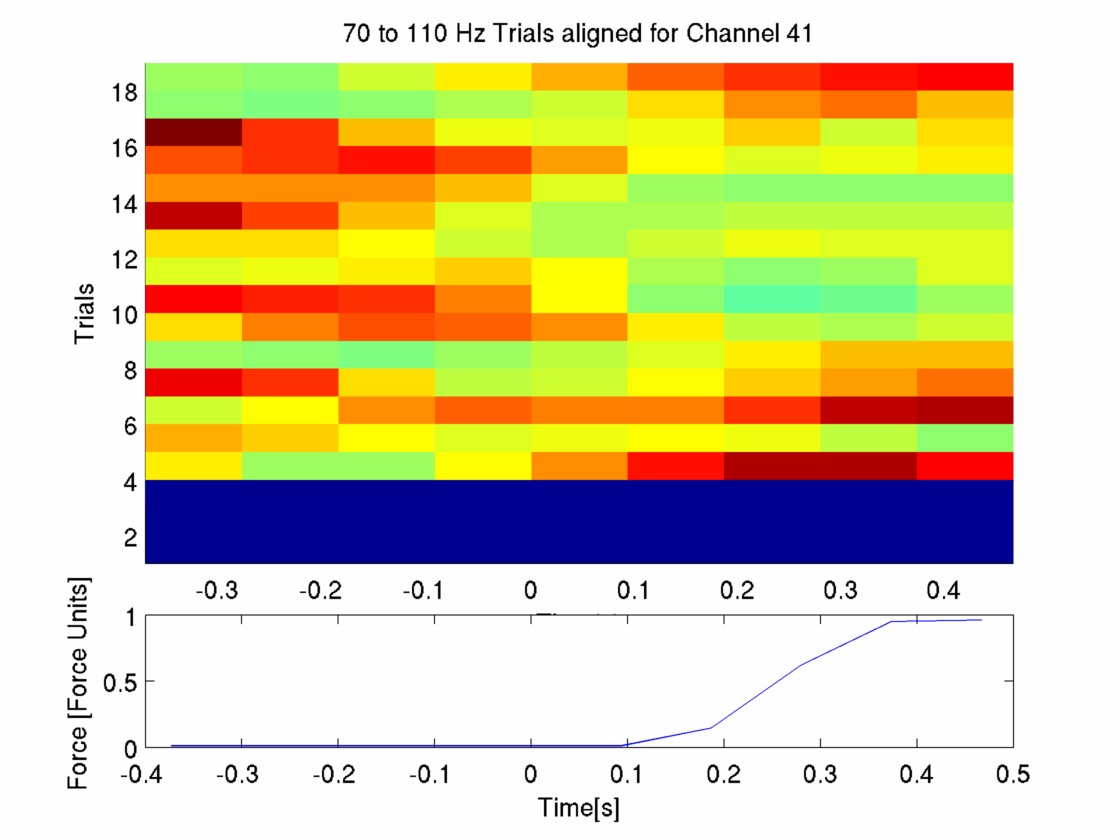
\includegraphics[scale=0.2]{plot_4_aligned_trials.png}

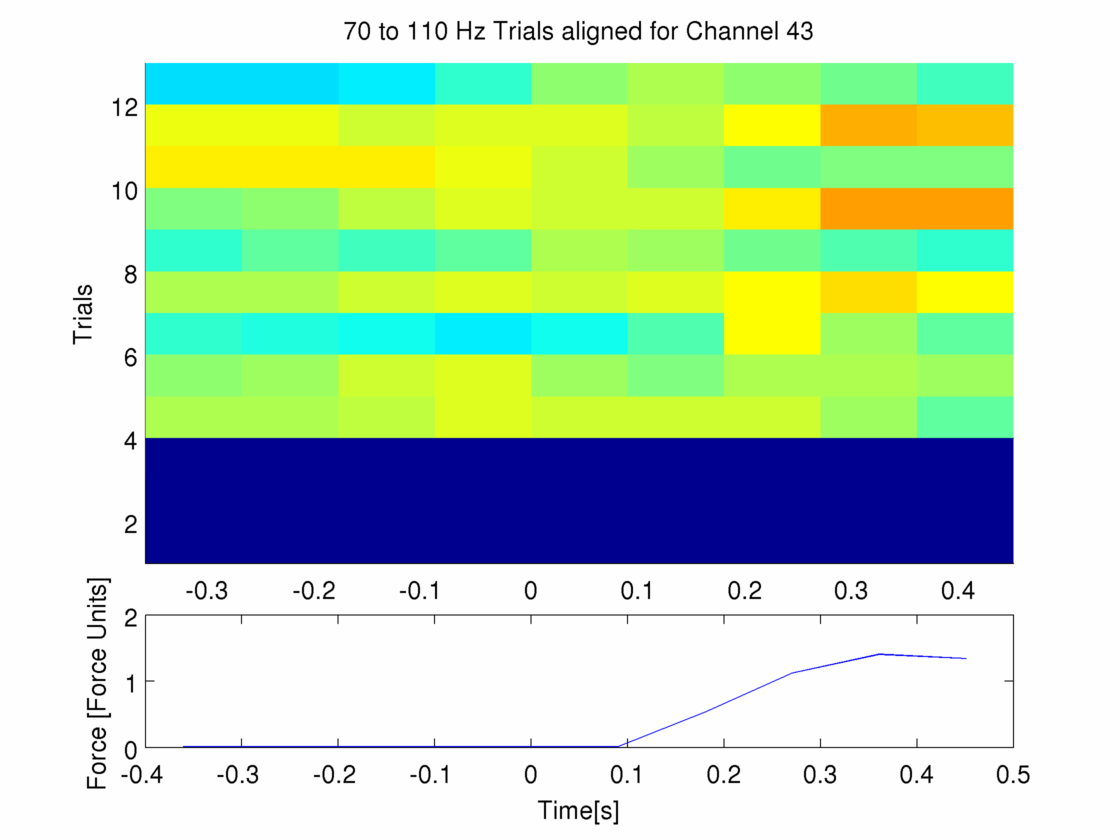
\includegraphics[scale=0.2]{plot_5_aligned_trials.png}
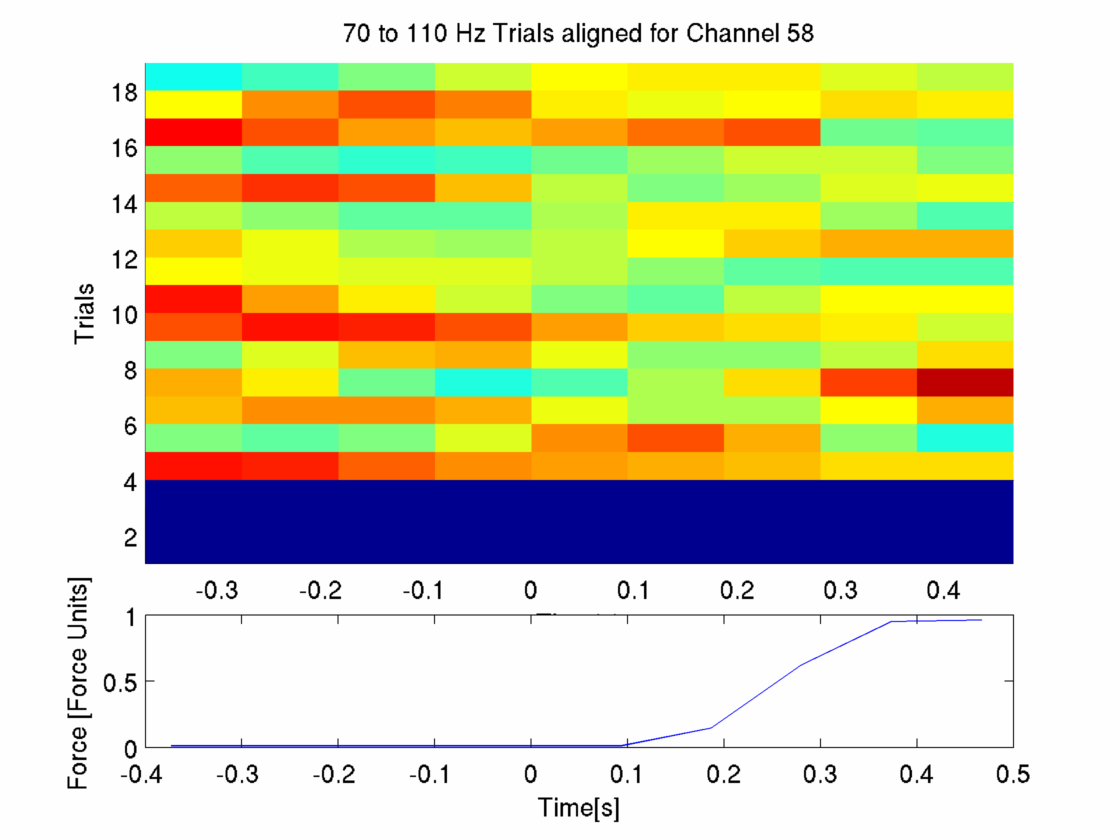
\includegraphics[scale=0.2]{plot_6_aligned_trials.png}



\end{document}